\documentclass[12pt]{article}

\pagestyle{empty}
\setlength{\topmargin}{0in}
\setlength{\headheight}{0in}
\setlength{\topsep}{0in}
\setlength{\textheight}{9in}
\setlength{\oddsidemargin}{0in}
\setlength{\evensidemargin}{0in}
\setlength{\textwidth}{6.5in}

\usepackage{palatino,graphics,amsmath,amssymb,enumitem}

\newcommand{\ds}{\displaystyle}
\newcommand{\vs}[1]{\vspace{#1in}}
\renewcommand{\vss}[1]{\vspace*{#1in}}
\newcommand{\bvec}{{\mathbf b}}
\newcommand{\cvec}{{\mathbf c}}
\newcommand{\dvec}{{\mathbf d}}
\newcommand{\evec}{{\mathbf e}}
\newcommand{\fvec}{{\mathbf f}}
\newcommand{\qvec}{{\mathbf q}}
\newcommand{\uvec}{{\mathbf u}}
\newcommand{\vvec}{{\mathbf v}}
\newcommand{\wvec}{{\mathbf w}}
\newcommand{\xvec}{{\mathbf x}}
\newcommand{\yvec}{{\mathbf y}}
\newcommand{\zvec}{{\mathbf y}}
\newcommand{\zerovec}{{\mathbf 0}}
\newcommand{\real}{{\mathbb R}}
\newcommand{\twovec}[2]{\left[\begin{array}{r}#1 \\ #2
    \end{array}\right]}
\newcommand{\ctwovec}[2]{\left[\begin{array}{c}#1 \\ #2
   \end{array}\right]}
\newcommand{\threevec}[3]{\left[\begin{array}{r}#1 \\ #2 \\ #3
  \end{array}\right]}
\newcommand{\cthreevec}[3]{\left[\begin{array}{c}#1 \\ #2 \\ #3
    \end{array}\right]}
\newcommand{\fourvec}[4]{\left[\begin{array}{r}#1 \\ #2 \\ #3 \\ #4
    \end{array}\right]}
\newcommand{\cfourvec}[4]{\left[\begin{array}{c}#1 \\ #2 \\ #3 \\ #4
    \end{array}\right]}
\newcommand{\mattwo}[4]{\left[\begin{array}{rr}#1 & #2 \\ #3 & #4 \\ \end{array}\right]}
\renewcommand{\span}[1]{\text{Span}\{#1\}}
\newcommand{\bcal}{{\cal B}}
\newcommand{\ccal}{{\cal C}}
\newcommand{\scal}{{\cal S}}
\newcommand{\wcal}{{\cal W}}
\newcommand{\ecal}{{\cal E}}
\newcommand{\coords}[2]{\left\{#1\right\}_{#2}}
\newcommand{\gray}[1]{\color{gray}{#1}}
\newcommand{\lgray}[1]{\color{lightgray}{#1}}
\newcommand{\rank}{\text{rank}}
\newcommand{\col}{\text{Col}}
\newcommand{\nul}{\text{Nul}}

\begin{document}

\noindent
{\bf Mathematics 227} \\ 
{\bf Dynamical systems}

\bigskip
For each of the following matrices, determine whether the associated
dynamical system is a repellor, saddle, or attractor.  Sketch the
eigenspaces and some trajectories to indicate the behavior of the
system below. 

\begin{enumerate}
\item
  $A =
  \left[
    \begin{array}{cc}
      1.3 & 0.2 \\
      0.2 & 1.3 \\
    \end{array}
  \right].
  $

  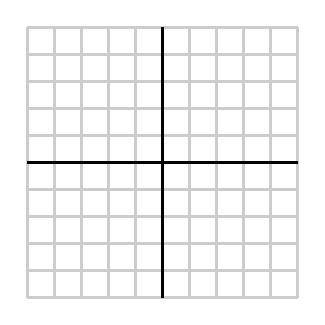
\includegraphics{empty.eps}


\item
  $A =
  \left[
    \begin{array}{cc}
      0.3 & 0.6 \\
      -0.6 & 1.8 \\
    \end{array}
  \right].
  $

  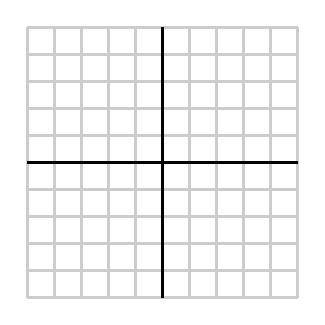
\includegraphics{empty.eps}
  
\item
  $A =
  \left[
    \begin{array}{cc}
      0.7 & -0.4 \\
      -0.1 & 0.7 \\
    \end{array}
  \right].
  $

  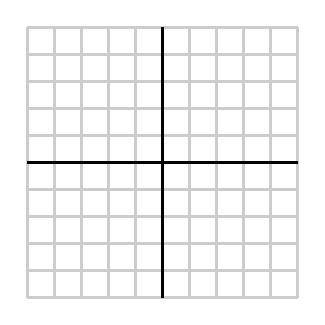
\includegraphics{empty.eps}

\item Suppose we have two species $R$ and $S$ that interact with one
  another and that we record the change in their populations from year
  to year. When we begin our study, the populations, measured in
  thousands, are $R_0$ and $S_0$; after $k$ years, the populations are
  $R_k$ and $S_k$.

  Knowing the populations in one year, we find their populations the
  next year:
  $$
  \begin{aligned}
    R_{k+1}&= 0.9R_k + 0.8S_k \\
    S_{k+1}&= 0.2R_k + 0.9S_k. \\
  \end{aligned}
  $$
  We will combine the populations into a vector
  $\xvec_k=\twovec{R_k}{S_k}$ and write
  $\xvec_{k+1}=A\xvec_k$ where
  $$
  A =
  \left[
    \begin{array}{cc}
      0.9 & 0.8 \\
      0.2 & 0.9 \\
    \end{array}
  \right].
  $$

  Classify this dynamical system as an attractor, repellor, or
  saddle and sketch some trajectories below.

  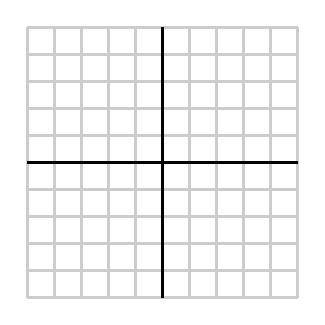
\includegraphics{empty.eps}

  Suppose that $\xvec_0=\twovec23$.  Write $\xvec_0$ as a linear
  combination of eigenvectors of $A$.

  \vs{1}
  Write the vectors $\xvec_1$, $\xvec_2$, and $\xvec_3$ as a linear
  combination of eigenvectors of $A$.

  \vs{1}
  \newpage
  When $k$ becomes very large, what happens to the ratio of the
  population $R_k/S_k$?

  \vs{1}
  After a long time, by approximately what factor does the population
  of $R$ grow every year?  By approximately what factor does the
  population $S$ grow every year?

  \vs{1}

\item Consider the dynamical system defined by the matrix
  $$
  A =
  \left[
    \begin{array}{cc}
      0.8 & 0.4 \\
      0.2 & 0.6 \\
    \end{array}
  \right].
  $$

  Find the eigenvalues and eigenvectors of $A$.

  \vs{1.5}
  Using the basis $\bcal$ of eigenvectors, sketch the trajectories in
  the $\bcal$-coordinate system on the left and the trajectories of
  the dynamical system on the right.

  \begin{center}
    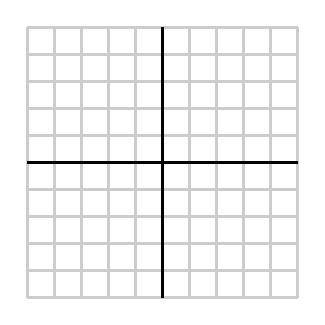
\includegraphics{empty.eps}
    \hspace*{24pt}
    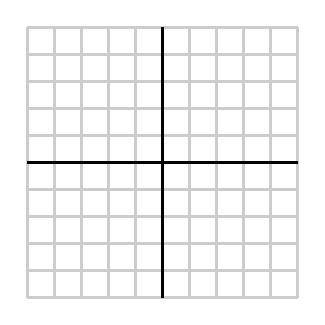
\includegraphics{empty.eps}
  \end{center}
  
  

\end{enumerate}


\end{document}
